\documentclass[a4paper,english,fleqn]{exam}

\usepackage{babel} % voor nederlandse afbreekregels e.d.
\usepackage{hyperref} % voor links, hier niet gebruikt
\usepackage{graphicx} % voor importeren van figures, hier niet gebruikt
\usepackage{tabularx} % voor tabellen met controle over kolombreedte, hier niet gebruikt
\usepackage{booktabs} % voor nettere tabellen dan de standaard
\usepackage{enumerate} % voor controle over nummering van items
\usepackage{amssymb,amsmath,amsthm,amsfonts} % van de AMS, voor nettere math
\usepackage{qtree} % voor het maken van mooie bomen, hier niet gebruikt
\usepackage{mathabx} %voor het \notdivides commando, niet gebruikt
\usepackage{adjustbox}
\usepackage{listings}
\usepackage{color}
\usepackage{pifont}
\usepackage{algorithm} % pseudocode
\usepackage[noend]{algpseudocode} %pseudocode 
\usepackage{sectsty}

\renewcommand\thesubsection{\thesection \alph{subsection}}
\newcommand{\s}{\text{*}}

%\DeclareGraphicsExtensions{.pdf,.png,.jpg}

\title{Emergent Architecture BEP}

\renewcommand{\baselinestretch}{0.9} 

\sectionfont{\fontsize{11}{15}\selectfont}

\renewcommand{\qedsymbol}{\hfill \emph{QED}}

% document variables:
\newcommand{\cMysename}{Model-based Optimization and Visualization of Aircraft Noise}
\newcommand{\doctitle}{Emergent Architecture}
\newcommand{\deadline}{2 May 2016}
\newcommand{\examdate}{\deadline}
\newcommand{\authors}{Elvan Kula \& Hans Schouten}
% ---

\newcommand{\cmark}{\ding{51}}%
\newcommand{\xmark}{\ding{55}}%

\newcommand{\itab}[1]{\hspace{0em}\rlap{#1}}
\newcommand{\tab}[1]{\hspace{.2\textwidth}\rlap{#1}}

% http://tex.stackexchange.com/questions/110328/formatting-a-logical-pd-derivation:
\newcommand{\fgh}[1]{\fvline%
  \makebox[0pt][l]{{%
      \raisebox{-1.4ex}[0pt][0pt]{\rule{#1}{\arrayrulewidth}}}}%
  \hspace*{\fitchindent}}
  
  \lstset{language=Java,
%alles tussen "//(*" en "*)" wordt als TeX code verIrkt
	escapeinside={//(*}{*)}} 
 


\newcommand*\xor{\mathbin{\oplus}}
% Fill these in:

% if you use algorithms, this is a nice one:
% http://www.lirmm.fr/~fiorio/AlgorithmSty/
%\usepackage[algo2e]{algorithm2e}

\makeatletter

\makeatother

%%%%%%%%%%%%%%%%%%%%%%%%%%%%%%%%%%%%%%%%%%%%%%%%%%%%%%%%%%%%%%%%%%%%%%%%%%%%%%%%
%% document start
%%%%%%%%%%%%%%%%%%%%%%%%%%%%%%%%%%%%%%%%%%%%%%%%%%%%%%%%%%%%%%%%%%%%%%%%%%%%%%%%
\begin{document}
\thispagestyle{empty}

\begin{center}

\vspace*{2cm}
{\huge \cMysename}

\begin{center}
    \line(1,0){450}
\end{center}

{\LARGE \doctitle}

\vspace{1cm}

{\Large \examdate}

\end{center}
\newpage

\tableofcontents
\newpage
%%%%%%%%%%%%%%%%%%%%%%%%%%%%%%%%%%%%%%%%%%%%%%%%%%%%%%%%%%%%%%%%%%%%%%%%%%%%%%%%
%% end of front page
%%%%%%%%%%%%%%%%%%%%%%%%%%%%%%%%%%%%%%%%%%%%%%%%%%%%%%%%%%%%%%%%%%%%%%%%%%%%%%%%

\section{Introduction}

\paragraph{Target Customers}
Aircraft and airport noise are complex subject matters which have been studied for decades and are still the focus of many research efforts nowadays. Also at the department of Air Transport \& Operations (ATO) at TU Delft’s Faculty of Aerospace Engineering. ATO has three research aims: 1) To develop radical new ways to optimize aircraft operations for efficiency, safety, cost and environmental impact; 2) To extend the analysis to an airline fleet and network level to include capacity and resilience; 3) To synthesize these to include operational safety at an airline and ATM level. To support their research findings at conferences, the researchers at ATO need a standalone application for model-based optimization and visualization of aircraft noise. This report summarizes the research phase of this project, during which we familiarize ourselves with the field and investigate what programming language, libraries, tools, etc. are best suited for our product.

\paragraph{Customer Needs}
We will provide a product that represents a creative and efficient way to minimize and visualize aircraft noise along simulated and real flight routes. This requires the implementation of two mathematical models: one for the computation of noise contours and one for the iterative optimization of aircraft trajectories for minimum noise and population annoyance. The models will be deployed by the research team to predict aircraft noise along a particular trajectory (flight route) and to update the trajectory design in an iterated manner to minimize the produced noise over populated areas around airports. Therefore, the parameters that take part in the optimization of aircraft trajectories range from the generic criterion of contour areas to a number of site-specific criteria based on the impact on population

Additionally, the program should be able to visualize the noise produced along the trajectory through a 3D animation pictured on a real map. This requires a visualization of noise contours, which are ‘noise footprints’ whose shape indicate areas of constant noise. Noise contours are a new subject to the research group and have not been implemented in relation with noise minimization before so this will be a challenging topic for us. The visualization should also show the effects of the produced aircraft noise on population annoyance.

In this orientation report we summarize the results of the research phase of this project as follows: first in Section 2 we give some more detailed information on the applications that we will extend and on similar products in the field. Section 3 focuses on the requirements gathering for this project, including a description of the various interviews we have conducted as well as the main requirements we identify. Section 4 then describes our chosen approach based on these requirements, including what programming language and tools we will use. Finally, Section 5 details what quality guarantees we will provide and how these are verified.
\section{Design Goals}
When designing the product we take the following design goals in consideration:

\textbf{Broad usage} \\
We try to make the program as broad as possible for usage by the ATO research department: the ATO researchers should be able to deploy the system for both simulated and real flight routes and they should be able to deploy the different models (noise model, optimization model, visualization model) of the program separately from each other. For each model the user should also have the option to turn on (or off) particular output, e.g. the user should be able to select particular contours to be show in Google Earth in the visualization component of the program.


\textbf{Modular}\\
Our goal is to split the program into different modules. Each model (noise, optimization and visualization) corresponds to one module. The different modules must be as loosely connected as possible so that for example changes within modules would not affect the graphical user interface (GUI) and vica versa.


\textbf{Quality of product}\\
We aim for the highest quality of the product. To achieve such a high quality we are going to build a good architecture for our program so that the code is easily maintained. We write automatic Unit test cases, so that if we make an enhancement to our program it automatically checks whether we have not broken another part of the code. We aim for a minimum line coverage of 75\%. We will couple the continuous integration server Jenkins to our Version Control System (VCS) in order to make sure that the code on the master branch always compiles and passes all the tests.

\textbf{User friendliness}\\
Another goal is to create an easy to use interface for the user, which is partly dependent on the overall quality of the program. We think that the modularity helps to guide the user through a work flow that works well for data analysis and visualization.

\textbf{Performance} \\
The data analysis should be performed within a reasonable period of time with a limit of ten seconds. When the results are calculated, the output should be shown directly on screen to ensure that the users don't experience long loading times. During analysis the program shows the user that it is still responding, but busy with doing a calculation. Also, a form of error management including error prevention and error correction (with error messages) is implemented in all layers of the architecture.

\textbf{Scalability and flexibility}\\
The program is able to process large sets of data with sizes in the gigabyte range and all models should respond within second(s).

\textbf{Use of Design Patterns} \\
We implemented our application following the Model-View-Presenter (MVP) pattern to separate the backend logic from the frontend that represents the program. This enables us to divide domain objects from the GUI elements to keep the code cleaner and the system more maintainable.

\section{Software Architecture Views}
This chapter describes what our software architecture looks like. First the subsystems are identified and explained. Then the software to hardware mapping is explained, followed by how we store persistent data. Lastly concurrency between information is explained.

\subsection{Design Principle: Separation of Concerns}
Following the design principle of Separation of Concerns for separating a computer program into distinct sections, we decided to implement the three models in such a way that they can be used as separate executables. They will be connected with each other in a pipelined manner in the main tab of the program to make them part of the workflow of the program. But these models can also be seen as standalone application: by specifying a dataset and wanted output you could also use the models outside of our program.
 
\subsection{Hardware Software Mapping}

Our program is designed for a single computer. The program also runs as one process. However, in future extensions we would like to make the program multi threaded. This would enable the user to run the optimization and visualization models in separate threads. This way the program will be able to optimize the entered flight trajectory while already visualizing the noise contours of the original (unoptimized) trajectory.
Also reading in the files could be put into a separate thread. This means that all the identifiers that are read could be shown in the select tab, the moment the thread reads them.

\subsection{Persistent data management}

For this program it is not required to store information persistently. The output of the program is stored as a KML file for visualization. The format of the output is structured in such a way that it can directly be entered into Google Earth and different visualization objects can be turned on or off in Google Earth.

The state of the program can also be stored easily by saving the intermediate results of the pipeline. For example, the output of the noise model or the optimization model can be stored as a .csv file to be read in at a later point in time. This can be stored in a user specified directory. After the file is loaded in the program, the program will be able to continue where the user left off. This also means that changes to intermediate results, that will be entered as input into the next model in the pipeline, will not require changes to the input file you used at the beginning. More on this can be found in section 2j. External Major Technologies.
 
Lastly, the possibility to store the KML files for visualization also enables the user to visualize multiple flight routes in Google Earth at the same time.

\subsection{Concurrency}
This subchapter is meant to describe how concurrency issues are solved. Because it is not possible that the program is used by multiple people at the same time and the data analysis is not divided over different processes, there are no concurrency issues. However, when multiple threads are going to be used in future projects, it becomes very important to think about concurrency. This could be useful when an ATO researcher wants to read in the next flight trajectory while the previous trajectory is still being optimized or visualized in the program. Our client let us know that this is not one of his requirements.

\newpage 

\subsection{Diagram of the architecture}

Here is a diagram of our layered architecture and the connection between the front-end and the back-end: \\

\begin{center}
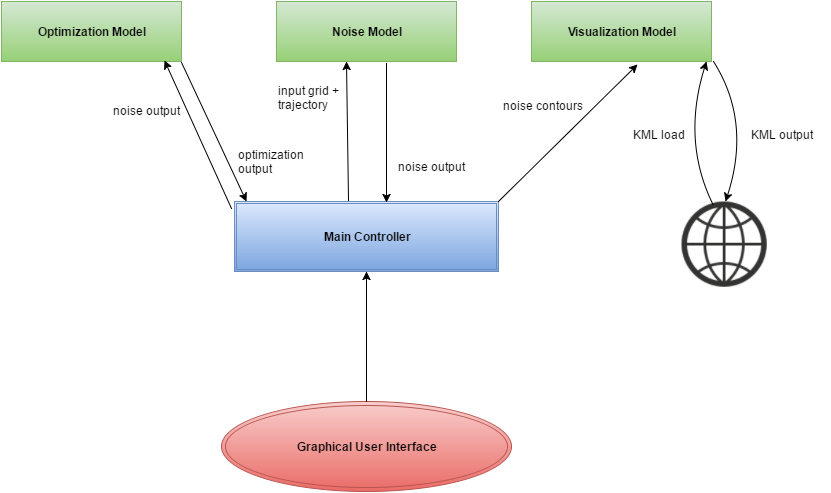
\includegraphics[width= 0.75\textwidth]{images/EmergentArchitecture} \\
\end{center}

As depicted in the diagram above, the models present the subsystems described in the Subsystem Decomposition section of the first chapter. They will exchange their outputs with the main controller which uses the output of one system as input for the next one. The main controller relegates the output of the optimization model as input to the noise model, and the output of the noise model to the visualization model. This way the models are executed in a pipelined manner. But given the right input files, the subsystems can also be run separately from each other and function as standalone applications.
The diagram also shows the connection between the frond-end and back-end of the system. Each subsystem contains an import component that collaborates with an import controller which controls the view of the noise, optimization and visualization tabs in the GUI. This is where the user specifies which data files he or she wants to import. 

\section{Major external technologies}

\textbf{Model View Controller} 

We decided to implement our project following the Model View Presenter (MVP) pattern. 

%The most important advantage of MVC is that it separates logic from the program's views. It's really helpful to use an architecture that utilizes a controller if there is logic required that doesn't necessarily fit into a model. In our case we are using a main controller which connects The advantages below convinced us to use MVC:


%\begin{itemize}
%\item First of all, MVC makes the code more clean and maintainable. It enables us to keep a good overview of the code.


%\item Because of the separation of concerns, the model and controller code could be reintegrated in other systems such as a web app, a desk app, a service without much effort.


%\item MVC enables us as a team to work in parallel. As an individual programmer you would probably have a different approach for the implementation but when working in a team, you will first need to discuss and agree on the structure of the code. With MVC the responsibilities of the developers can be easily divided and assigned.

%\end{itemize}

%From a Model View Controller perspective, the files constructing the GUI will correspond to the view. The controller exists of a main method (shell script) which connects and executes the models in a pipelined manner. It takes a trajectory and grid as input and will return the corresponding KML files to visualize the (optimized) trajectory with noise contours in Google Earth. In our case there are three models: noise model, optimization model and visualization model. These models will be connected to the view through the controller. The way we applied MVC in our architecture can be seen in the diagram below.

%[TO BE UPDATED]

%\underline{Alternatives to MVC}

%Other architectural patterns that could be used in our situation are for example Presentation-abstraction-control, Model View Presenter, and Model View ViewModel. These patterns are interaction-oriented and similar to MVC.
 
%An important difference with Presentation-abstraction-control (PAC) is the abstraction component. PAC retrieves and processes the data with the Abstraction component and makes a visual presentation of the data (a template actually) with the Presentation component. The Presentation and Abstraction components never speak to each other. This communication and control flow between these components are all handled by the Control component. This is also the reason why the PAC doesn't suit our system. PAC is only useful when you aren't calling your data store directly from your display layer, which is actually what we want to do in our system. The user needs to be able to import specified files in the user interface.
 
%Model View Presenter (MVP) and Model View ViewModel (MVVM) are derivations of the MVC pattern. In MVP the controller has been replaced by a Presentation component to which all presentation logic is pushed. In MVVM this is pushed to the ViewModel. These components are responsible for exposing methods and handling all UI events by receiving input from users via the View, then process the user's data with the help of Model and passing the results back to the View. Unlike View and Controller, View and Presenter or ViewModel are completely decoupled from each other and their communication is handled through the interface. These patterns have a clean separation of the View and Model and the amount of data is reduced because of a passive View. However, this also means that there is less encapsulation and more work to do as the developer has to do all the data binding himself. We preferred MVC above these patterns because we wanted our View to process the input partially before passing it to the next layer. This is needed to pass on the output from the noise model to the optimization model.


\end{document}
%%%%%%%%%%%%%%%%%%%%%%%%%%%%%%%%%%%%%%%%%%%%%%%%%%%%%%%%%%%%%%%%%%%%%%%%%%%%%%%%